
\fullcite{zhym12}


\begin{multicols}{2}
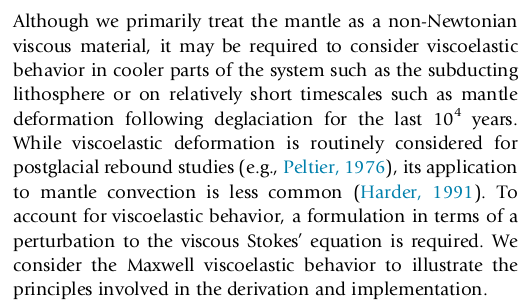
\includegraphics[width=8.25cm]{images/viscoelasticity/zhym12_a}
\end{multicols}

\begin{multicols}{2}
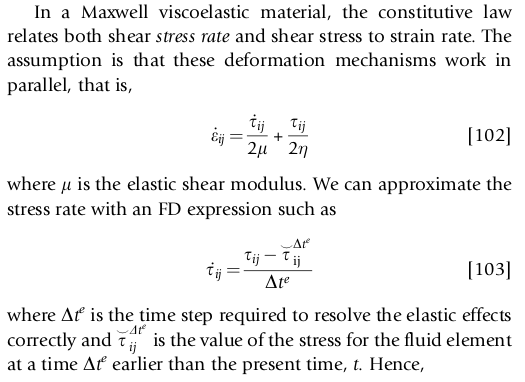
\includegraphics[width=8.25cm]{images/viscoelasticity/zhym12_b}\\
\[
\dot{\bm\varepsilon} = \frac{ \dot{\bm \tau}  }{2\mu} + \frac{{\bm \tau}}{2\eta} 
\]
\end{multicols}

\begin{multicols}{2}
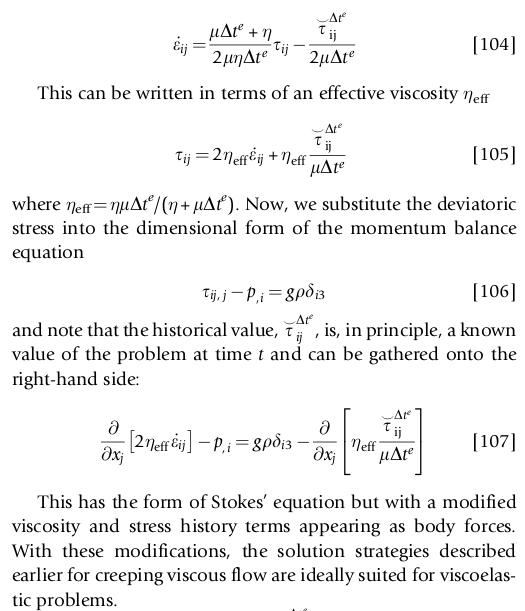
\includegraphics[width=8.25cm]{images/viscoelasticity/zhym12_c}\\
\[
\dot{\bm\varepsilon} = \frac{\mu \delta t^e + \eta}{2 \mu \eta \delta t^e} {\bm \tau}
- ... 
\]
\[
{\bm \tau} = 2 \eta_{ve} \dot{\bm\varepsilon} + \frac{\eta_{ve} {\bm \tau}^{before} }{\mu \delta t^e}
\]
\[
\eta_{ve}=\frac{\eta\mu \delta t^e}{\eta + \mu \delta t^e}
\]
\[
\vec\nabla \cdot (2 \eta_{ve} \dot{\bm\varepsilon}) - \vec\nabla p
=
\rho \vec{g}
-\vec\nabla \cdot(\eta_{ve}\frac{1}{\mu \delta t^e} ... )
\]
\end{multicols}

\begin{multicols}{2}
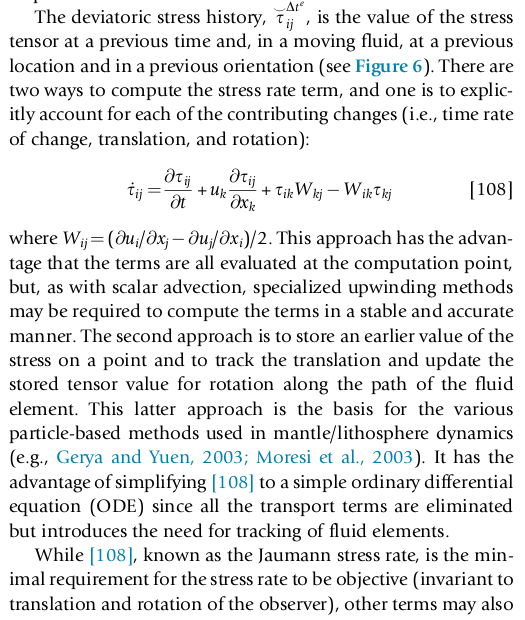
\includegraphics[width=8.25cm]{images/viscoelasticity/zhym12_d} \\
\[
{\bm \tau} = \frac{\partial {\bm \tau}}{\partial t} + 
(\vec\upnu \cdot \vec\nabla ){\bm \tau} + 
{\bm \tau} \cdot \dot{\bm\omega} - \dot{\bm\omega} \cdot {\bm\tau}
\]
\end{multicols}

\begin{multicols}{2}
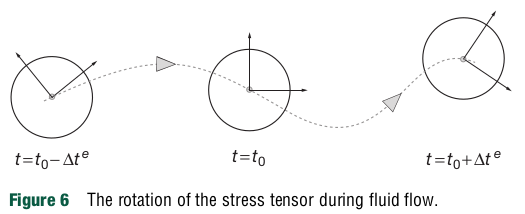
\includegraphics[width=8.25cm]{images/viscoelasticity/zhym12_e}
\end{multicols}

\begin{multicols}{2}
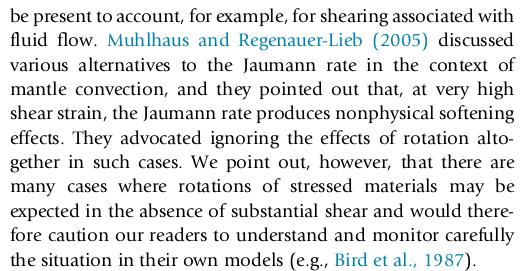
\includegraphics[width=8.25cm]{images/viscoelasticity/zhym12_f}
\end{multicols}

\begin{multicols}{2}
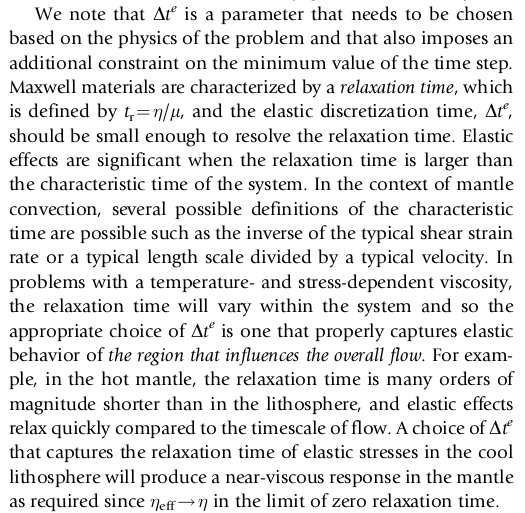
\includegraphics[width=8.25cm]{images/viscoelasticity/zhym12_g}
\end{multicols}

\begin{multicols}{2}
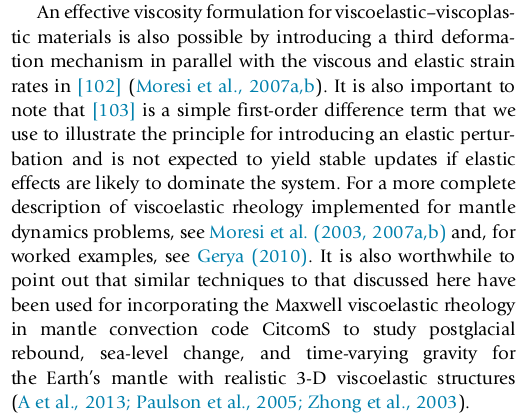
\includegraphics[width=8.25cm]{images/viscoelasticity/zhym12_h}
\end{multicols}
